\documentclass[xcolor=dvipsnames,aspectratio=169,t]{beamer}
  % t means frames are vertically centered to the top
\usepackage{slides-header}
\title{Applications of Linear Systems}

\begin{document}
\maketitle

\begin{frame}{Balancing Chemical Equations}
  In a chemical reaction, molecules recombine to produce other molecules.
  
  The same \colorb{number} and \colorb{type} of atoms are present at the beginning and end of the reaction.
  \bigskip
  
  Consider the burning of methane:
  $ \mathrm{C}\mathrm{H}_4 + \mathrm{O}_2 \rightarrow 
    \mathrm{C}\mathrm{O}_2 + \mathrm{H}_2 \mathrm{O}$.
    
  \vspace*{3em}
  
  \pause
  We thus have the \alert{balanced} chemical equation 
  $ \mathrm{C}\mathrm{H}_4 + \colorb{2}\mathrm{O}_2 \rightarrow 
    \mathrm{C}\mathrm{O}_2 + \colorb{2}\mathrm{H}_2 \mathrm{O}$.

\end{frame}


\begin{frame}{Network Flow}

  \begin{columns}
    \column{0.65\tw}
    {\small
  \bi
  \ii A \alert{network} consists of a set of points, called \alert{nodes} with lines, called \alert{branches} connecting some or all of the nodes.
  \ii The direction of the flow is indicated by each branch (are things flowing in or out of the node?).
  \ii The flow amount (or rate) is either given or denoted by a variable.
  \ii We assume the total flow into a network equals the total flow out of the network.
  \ii The goal is to determine the flow in each branch when partial information is known.
  \ii Network flows have applications to current flow through a circuit, flow of goods through supply chains, social networks, and \alert{urban planning} to name a few.
  \ei
    }
    
  \column{0.35\tw}

  
\includegraphics[width=0.95\tw]{images/fig-social-network.png}
  \smallskip
  
  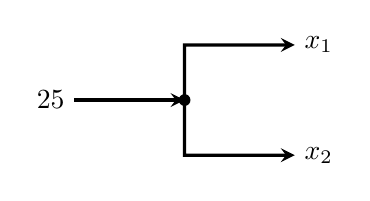
\begin{tikzpicture}[scale=.7]
    \node[anchor=east] (v) at (-2,0) {$25$};
    \node[anchor=west] (x1) at (2,1) {$x_1$};
    \node[anchor=west] (x2) at (2,-1) {$x_2$};
    \draw[very thick,-stealth] (v)--(0,0);
    \draw[very thick,-stealth] (0,0)--(0,1)--(x1);
    \draw[very thick,-stealth] (0,0)--(0,-1)--(x2);
    \node[circle,fill,inner sep=1.5pt] at (0,0) {};
  \end{tikzpicture}

  \end{columns}

  \end{frame}

\begin{frame}{Traffic Flow in Baltimore}

  The network in the figure shows the flow of traffic (in vehicles per hour) over several one way streets in downtown Baltimore during a typical early afternoon.
  Determine the general flow pattern for the network.

  \begin{columns}
  \column{0.4\tw}
  \vspace*{-2em}
  
  
% figure of traffic network

  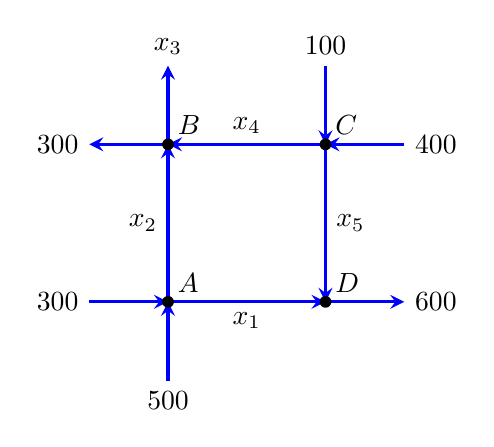
\begin{tikzpicture}
    \coordinate (A) at (-1,-1); \node[anchor=south west] at (A) {$A$};
    \coordinate (B) at (-1,1); \node[anchor=south west] at (B) {$B$};
    \coordinate (C) at (1,1); \node[anchor=south west] at (C) {$C$};
    \coordinate (D) at (1,-1); \node[anchor=south west] at (D) {$D$};
    \draw[very thick,blue,stealth-] (A)--node[pos=1,anchor=north,black] () {$500$} ++(0,-1);
    \draw[very thick,blue,stealth-] (A)--node[pos=1,anchor=east,black] () {$300$} ++(-1,0);
    \draw[very thick,blue,-stealth] (B)--node[pos=1,anchor=east,black] () {$300$} ++(-1,0);
    \draw[very thick,blue,-stealth] (B)--node[pos=1,anchor=south,black] () {$x_3$} ++(0,1);
    \draw[very thick,blue,stealth-] (C)--node[pos=1,anchor=south,black] () {$100$} ++(0,1);
    \draw[very thick,blue,stealth-] (C)--node[pos=1,anchor=west,black] () {$400$} ++(1,0);
    \draw[very thick,blue,-stealth] (D)--node[pos=1,anchor=west,black] () {$600$} ++(1,0);
    \draw[very thick,blue,-stealth] (A)--node[pos=.5,anchor=east,black] () {$x_2$} (B);
    \draw[very thick,blue,-stealth] (C)--node[pos=.5,anchor=south,black] () {$x_4$} (B);
    \draw[very thick,blue,-stealth] (A)--node[pos=.5,anchor=north,black] () {$x_1$} (D);
    \draw[very thick,blue,-stealth] (C)--node[pos=.5,anchor=west,black] () {$x_5$} (D);
    \node[circle,fill,inner sep=1.5pt] at (A) {};
    \node[circle,fill,inner sep=1.5pt] at (B) {};
    \node[circle,fill,inner sep=1.5pt] at (C) {};
    \node[circle,fill,inner sep=1.5pt] at (D) {};
  \end{tikzpicture}


  \column{0.6\tw}
  \begin{tabular}{crcl}
    \hline
    Intersection & Flow in & & Flow out\\
    \hline
    A & $300+500$ & $=$ & $x_1+x_2$\\
    B & $x_2 + x_4$ & $=$ & $300+x_3$\\
    C & $100+400$ & $=$ & $x_4+x_5$\\
    D & $x_1+x_5$ & $=$ & $600$\\
    \hline
  \end{tabular}

  \[
  \begin{array}{ccccccccccc}
    x_1 & + & x_2 &   &         &    &        &   &          &= & 800\\
           &     & x_2 & - & x_3 & + & x_4 &   &         &=& 300\\
           &     &        &    &        &    & x_4 & + & x_5 &=& 500\\
    x_1 &     &        &    &       &     &        & + & x_5 &=& 600\\
           &      &        &   & x_3 &    &        &     &        &=& 400
  \end{array}
  \]

  \end{columns}
   
  \end{frame}

\begin{frame}{Solving the System}

  We need to solve the following nonhomogeneous linear system of equations:

  \begin{columns}[T]
    \column{0.3\tw}
    
    \hspace*{2em}\scalebox{0.65}{
% figure of traffic network

  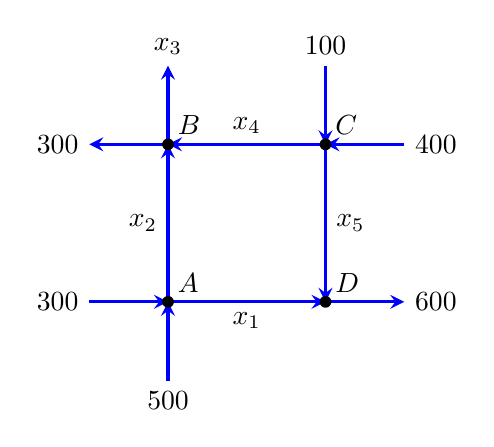
\begin{tikzpicture}
    \coordinate (A) at (-1,-1); \node[anchor=south west] at (A) {$A$};
    \coordinate (B) at (-1,1); \node[anchor=south west] at (B) {$B$};
    \coordinate (C) at (1,1); \node[anchor=south west] at (C) {$C$};
    \coordinate (D) at (1,-1); \node[anchor=south west] at (D) {$D$};
    \draw[very thick,blue,stealth-] (A)--node[pos=1,anchor=north,black] () {$500$} ++(0,-1);
    \draw[very thick,blue,stealth-] (A)--node[pos=1,anchor=east,black] () {$300$} ++(-1,0);
    \draw[very thick,blue,-stealth] (B)--node[pos=1,anchor=east,black] () {$300$} ++(-1,0);
    \draw[very thick,blue,-stealth] (B)--node[pos=1,anchor=south,black] () {$x_3$} ++(0,1);
    \draw[very thick,blue,stealth-] (C)--node[pos=1,anchor=south,black] () {$100$} ++(0,1);
    \draw[very thick,blue,stealth-] (C)--node[pos=1,anchor=west,black] () {$400$} ++(1,0);
    \draw[very thick,blue,-stealth] (D)--node[pos=1,anchor=west,black] () {$600$} ++(1,0);
    \draw[very thick,blue,-stealth] (A)--node[pos=.5,anchor=east,black] () {$x_2$} (B);
    \draw[very thick,blue,-stealth] (C)--node[pos=.5,anchor=south,black] () {$x_4$} (B);
    \draw[very thick,blue,-stealth] (A)--node[pos=.5,anchor=north,black] () {$x_1$} (D);
    \draw[very thick,blue,-stealth] (C)--node[pos=.5,anchor=west,black] () {$x_5$} (D);
    \node[circle,fill,inner sep=1.5pt] at (A) {};
    \node[circle,fill,inner sep=1.5pt] at (B) {};
    \node[circle,fill,inner sep=1.5pt] at (C) {};
    \node[circle,fill,inner sep=1.5pt] at (D) {};
  \end{tikzpicture}
}
    
      \column{0.7\tw}
\[   \begin{array}{ccccccccccc}
    x_1 & + & x_2 &   &         &    &        &   &          &= & 800\\
           &     & x_2 & - & x_3 & + & x_4 &   &         &=& 300\\
           &     &        &    &        &    & x_4 & + & x_5 &=& 500\\
    x_1 &     &        &    &       &     &        & + & x_5 &=& 600\\
           &      &        &   & x_3 &    &        &     &        &=& 400
\end{array} \]

\end{columns}
  \medskip

   We have an augmented matrix

   \[ \bbm
   $1$ & $1$ & $0$ & $0$ & $0$ & $800$\\
   $0$ & $1$ & $-1$ & $1$ & $0$ & $300$\\
   $0$ & $0$ & $0$ & $1$ & $1$ & $500$\\
   $1$ & $0$ & $0$ & $0$ & $1$ & $600$\\
   $0$ & $0$ & $1$ & $0$ & $0$ & $400$
   \ebm
   \sim
   \bbm
   $1$ & $0$ & $0$ & $0$ & $1$ & $600$\\
   $0$ & $1$ & $0$ & $0$ & $-1$ & $200$\\
   $0$ & $0$ & $1$ & $0$ & $0$ & $400$\\
   $0$ & $0$ & $0$ & $1$ & $1$ & $500$\\
   \ebm
   \rightarrow
   \left\{ \begin{array}{l}
     x_1=600-x_5\\
     x_2 = 200 + x_5\\
     x_3 = 400\\
     x_4 = 500-x_5\\
     x_5 \mbox{ is free}
     \end{array} \right.
   \]

\end{frame}

  \end{document}
